\documentclass[
10pt,
a4paper,
]{article}
\usepackage{eurosym,natbib,alifeconf,hyperref}
\usepackage[landscape,twocolumn]{geometry}
\title{The Pop Button}
\author{Kentin$^{1}$ \and Nil$^{2}$ }

\begin{document}
\maketitle

\section{In a word}

The pop button is a device that aim to be your daily companion for noting every furniture you need anytime you think about it


\section{Introduction}

The device needs a "rotate and push" button, a wi-fi module to communicate with a server, a screen, a battery holder and of course a PIC32 System on Chip 

\begin{table}[!hbt]
\center{
\begin{tabular}{|c|c|c|}\hline
component & price(\euro) & consumption\\ \hline\hline

\href{http://fr.farnell.com/microchip/pic32mx174f256b-i-so/mcu-32-bits-pic32mx-72mhz-soic/dp/2775021?st=PIC32MX174F256B}
{PIC32MX174F256B-I/SO} & 3.48 & $\sim$ 200mA \\

\href{http://fr.farnell.com/microchip/atwinc1500-mr210pb1952/mod-iot-smartconnect-2-472ghz/dp/2759346?st=atwin}
{ATWINC1500}  & 6.61 & 70mA / 172mA \\

\href{http://fr.farnell.com/midas/mccog128064b12w-fptlw/afficheur-lcd-graphique-128x64/dp/2664759}
{MCCOG128064B12W} & 8.69 & 40mA \\

\href{http://fr.farnell.com/bourns/pel12d-2226f-s3024/rotary-encoder-incremental-24/dp/1857558?st=rotary\%20encoder}
{PEL12D-2226F-S3024} & 1.88 & 10mA\\

\href{http://fr.farnell.com/optek-technology/opb732/capteur-reflectif-pcb/dp/1226877}
{OPB732} & 3.2 & 50mA\\

\hline
total & 23,87 & 370mA / 472mA\\
\hline
\end{tabular}
}
\caption{basic specifications}
\end{table}

\section{Block Diagram}
This is a basic block diagram describing the architecture of the device
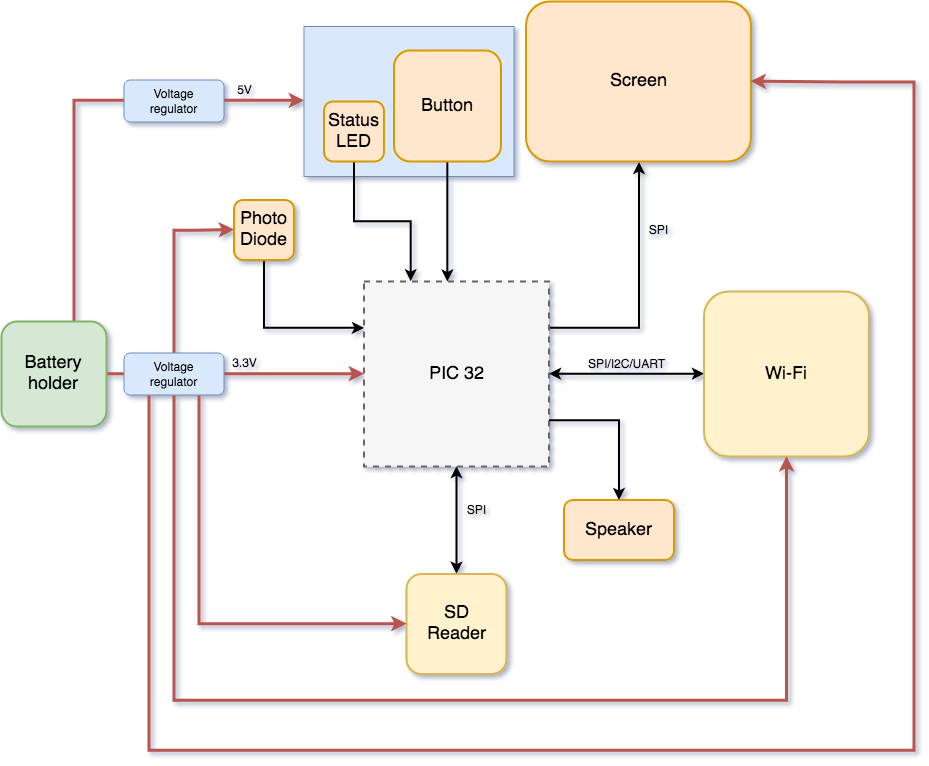
\includegraphics[width=3.7in]{block-diagram.png}

\section{How it works}
The principal purpose of the pop button is to choice in a list what we want to order for the next time you go to the shop or do your weekly/monthly order to you preferred provider

\begin{itemize}
    \item Thanks to his photodiode turning on the device can be accomplished by passing your hand in front of it or directly pushing the button once.
    \item Once the device is on you can see some items on the screen, you can easily change the current item by turning the rotary button, once you found the desired item you push the button and it will light up green or red depending on the possibility to order your choice.
    \item The list is composed on the server and sent to the device thanks to his wi-fi module, it is stored in the sd card so the list can be long 
    \item In order to connect the device to your network you can either use the SDcard to change the configuration file with your computer or long push the button and enter the password within a appropriate menu using the button
\end{itemize}

\footnotesize
\bibliographystyle{apalike}
\bibliography{sample}
{
\mbox{}\\
$^1$qdurot \\
$^2$nburcion \\
}

\end{document}